%
% Matrixzerlegungen
%
% (c) 2009 Prof Dr Andreas Mueller, Hochschule Rapperswil
%
\chapter{Matrixzerlegungen\label{chapter-zerlegung}}
\rhead{Matrixzerlegungen}
Der Gauss-Algorithmus löst nicht nur Gleichungssysteme, er berechnet
auch die inverse Matrix oder die Determinante.
Für viele Zwecke ist
aber die Berechnung der Inversen nicht unbedingt notwendig, es reicht,
wenn eine gegebenen Matrix $A$ in Faktoren $A=BC$ zerlegt werden kann,
wobei die Faktoren $B$ und $C$ besondere Eigenschaften haben sollen.
Um ein Gleichungssystem
\[
Ax=b
\]
zu lösen, müssen dann zwei Gleichungssysteme Systeme
\begin{align*}
Cy&=b\\
Bx&=y
\end{align*}
gelöst werden, was trotzdem eine Vereinfachung sein kann, wenn
$B$ und $C$ besonders einfach zu invertieren sind.
Oder die Berechnung der Determinanten kann mit Hilfe der Formel
\[
\det(A)=\det(B)\det(C)
\]
vereinfacht werden, sofern die Matrizen $B$ oder $C$ einfach
zu berechnende Determinanten haben.

%
% dreieck.tex
%
% (c) 2009 Prof Dr Andreas Mueller, Hochschule Rapperswil
%
\section{Zerlegung von Dreiecksmatrizen}
\index{Dreiecksmatrix}
Als Vorbereitung untersuchen wir einige Beispiele von möglichen
Zerlegungen von Dreiecksmatrizen.
In diesem Abschnitt ist $L$ immer eine untere Dreiecksmatrix
\[
L=\begin{pmatrix}
l_{11}&0     &\dots &0     \\
l_{21}&l_{22}&\dots &0     \\
\vdots&\vdots&\ddots&\dots \\
l_{n1}&l_{n2}&\dots &l_{nn}
\end{pmatrix}
\]
\begin{hilfssatz}
Eine untere Dreiecksmatrix $L$ kann als Produkt einer Diagonalmatrix
mit einer unteren Dreiecksmatrix $L_0$ mit Einsen auf der Diagonalen
geschrieben werden, $L=\operatorname{diag}(l_{11},\dots,l_{nn}) L_0$.
\end{hilfssatz}

\begin{proof}[Beweis]
Für $L_0$ muss man die Matrix
\begin{align*}
L_0&=
\operatorname{diag}(l_{11},\dots,l_{nn})^{-1} L
=
\begin{pmatrix}
\frac1{l_{11}}&0             &\dots &0\\
0             &\frac1{l_{22}}&\dots &\vdots\\
\vdots        &\vdots        &\ddots&\vdots\\
0             &0             &\dots &\frac1{l_{nn}}
\end{pmatrix}
\begin{pmatrix}
l_{11}&0     &\dots &0     \\
l_{21}&l_{22}&\dots &0     \\
\vdots&\dots &\ddots&\dots \\
l_{n1}&l_{n2}&\dots &l_{nn}
\end{pmatrix}
\\
&=
\begin{pmatrix}
\frac{l_{11}}{l_{11}}&0                    &\dots &0     \\
\frac{l_{21}}{l_{22}}&\frac{l_{22}}{l_{22}}&\dots &0     \\
\vdots               &\vdots               &\ddots&\vdots\\
\frac{l_{n1}}{l_{nn}}&\frac{l_{n2}}{l_{nn}}&\dots &\frac{l_{nn}}{l_{nn}}
\end{pmatrix}
=
\begin{pmatrix}
1                    &0                    &\dots &0     \\
\frac{l_{21}}{l_{22}}&1                    &\dots &0     \\
\vdots               &\vdots               &\ddots&\vdots\\
\frac{l_{n1}}{l_{nn}}&\frac{l_{n2}}{l_{nn}}&\dots &1
\end{pmatrix}
\end{align*}
nehmen.
\end{proof}
Offenbar entsteht $L_0$ aus $L$, indem man jede Zeile durch das zugehörige
Diagonalelement teilt, ähnlich wie man das im Laufe des Gauss-Algorithmus
macht.

\begin{hilfssatz}
Sei $L$ eine unter Dreiecksmatrix mit $n$ Zeilen und Spalten, und $k<n$.
Dann kann man $L$ in zwei untere Dreiecksmatrizen aufteilen:
\begin{align*}
L&=
\begin{pmatrix}
l_{11}   &\dots &0        &0          &\dots &0     \\
\vdots   &\ddots&\vdots   &\vdots     &\ddots&\vdots\\
l_{k1}   &\dots &l_{kk}   &0          &\dots &0     \\
l_{k+1,1}&\dots &l_{k+1,k}&l_{k+1,k+1}&\dots &0     \\
\vdots   &\ddots&\vdots   &\vdots     &\ddots&\vdots\\
l_{nn}   &\dots &l_{nk}   &l_{n,k+1}  &\dots &l_{nn}
\end{pmatrix}
\\
&=
\begin{pmatrix}
l_{11}   &\dots &0        &0          &\dots &0     \\
\vdots   &\ddots&\vdots   &\vdots     &\ddots&\vdots\\
l_{k1}   &\dots &l_{kk}   &0          &\dots &0     \\
l_{k+1,1}&\dots &l_{k+1,k}&1          &\dots &0     \\
\vdots   &\ddots&\vdots   &\vdots     &\ddots&\vdots\\
l_{nn}   &\dots &l_{nk}   &0          &\dots &1
\end{pmatrix}
\begin{pmatrix}
1        &\dots &0        &0          &\dots &0     \\
\vdots   &\ddots&\vdots   &\vdots     &\ddots&\vdots\\
0        &\dots &1        &0          &\dots &0     \\
0        &\dots &0        &l_{k+1,k+1}&\dots &0     \\
\vdots   &\ddots&\vdots   &\vdots     &\ddots&\vdots\\
0        &\dots &0        &l_{n,k+1}  &\dots &l_{nn}
\end{pmatrix}
\end{align*}
\end{hilfssatz}

\begin{proof}[Beweis]
Durch Nachrechnen.
\end{proof}

Diese Zerlegung kann man natürlich iterieren, bis in jeder Teilmatrix
nur noch eine Spalte übrig bleibt.
Schreiben wir
\[
L_i=\begin{pmatrix}
1      &\dots &0     &\dots &0     \\
\vdots &\ddots&\vdots&\ddots&\vdots\\
0      &\dots &l_{ii}&\dots &0     \\
\vdots &\ddots&\vdots&\ddots&\vdots\\
0      &\dots &l_{ni}&\dots &1
\end{pmatrix},
\]
dann können wir $L$ schreiben als
\begin{equation}
L=L_1L_2\dots L_{n-1}L_n.
\label{lproductdecomposition}
\end{equation}


%
% lr.tex -- Zerlegung in Dreiecksmatrizen
%
% (c) 2009 Prof Dr Andreas Mueller, Hochschule Rapperswil
%
\section{Zerlegung einer Matrix in Dreiecksmatrizen}
\rhead{Zerlegung einer Matrix in Dreiecksmatrizen}
\index{LU-Zerlegung}
\index{Zerlegung!LU}
Der Gauss-Algorithmus produziert mit bei der Vorwärtsreduktion eine
obere Dreiecksmatrix, die noch dazu lauter Einsen auf der Diagonalen
hat.
Es liegt also nahe, eine Zerlegung von $A$ mit dieser Dreiecksmatrix
als Faktor $U$ zu versuchen.

Um den zweiten Faktor zu finden, studieren wir nochmals den
Gauss-Algorithmus.
Im $k$-ten Schritt wird das Diagonalelement
$a_{kk}$ zu $1$ gemacht, und damit werden alle Elemente späteren
Elemente in der Spalte eliminiert.
Man weiss also bereits, was an
diesen Stellen in der Matrix stehen wird, es ist nicht nötig, diese
Einträge zu berechnen oder zu speichern.
Wir lassen daher diese Einträge stehen.
Das Gauss-Tableau sieht dann nach der Vorwärtsreduktion
so aus:
\[
\begin{tabular}{|>{$}c<{$}>{$}c<{$}>{$}c<{$}>{$}c<{$}>{$}c<{$}|}
\hline
a_{11}&a_{12}&a_{13}&\dots &a_{1n}\\
a_{21}&a_{22}&a_{23}&\dots &a_{2n}\\
a_{31}&a_{32}&a_{33}&\dots &a_{3n}\\
\vdots&\vdots&\vdots&\ddots&\vdots\\
a_{n1}&a_{n2}&a_{n3}&\dots &a_{nn}\\
\hline
\end{tabular}
\rightarrow
\begin{tabular}{|>{$}c<{$}>{$}c<{$}>{$}c<{$}>{$}c<{$}>{$}c<{$}|}
\hline
l_{11}&u_{12}&u_{13}&\dots &u_{1n}\\
l_{21}&l_{22}&u_{23}&\dots &u_{2n}\\
l_{31}&l_{32}&l_{33}&\dots &u_{3n}\\
\vdots&\vdots&\vdots&\ddots&\vdots\\
l_{n1}&l_{n2}&l_{n3}&\dots &l_{nn}\\
\hline
\end{tabular}
\]
Zu beachten ist ferner, dass der Gauss-Algorithmus im $k$-ten Schritt nur 
die Elemente in den Zeilen mit Indices $\ge k$ und Spalten mit Indices $>k$ 
modifiziert.
Die beiden Matrizen $L$ und $R$ sind dann
\[
L=\begin{pmatrix}
l_{11}&0     &0     &\dots &0\\
l_{21}&l_{22}&0     &\dots &0\\
l_{31}&l_{32}&l_{33}&\dots &0\\
\vdots&\vdots&\vdots&\ddots&\vdots\\
l_{n1}&l_{n2}&l_{n3}&\dots &l_{nn}
\end{pmatrix},
\qquad
U=
\begin{pmatrix}
1     &u_{12}&u_{13}&\dots &u_{1n}\\
0     &1     &u_{23}&\dots &u_{2n}\\
0     &0     &1     &\dots &u_{3n}\\
\vdots&\vdots&\vdots&\ddots&\vdots\\
0     &0     &0     &\dots &1
\end{pmatrix}.
\]
Wir wissen bereits aus (\ref{lproductdecomposition}), dass sich $L$
ein Produkt von Matrizen $L_i$ zerlegen lässt, die jeweils nur
die $i$-te Spalte von $L$ enthalten, im übrigen aber wie eine Einheitsmatrix
aussehen.

Wir behaupten jetzt, dass $L_i$ den $i$-ten Gauss-Vorwärtsredutionsschritt
rück\-gängig macht.
Da $U$ das Resultat der Vorwärtsreduktion ist, 
muss $LU$ die ursprüngliche Matrix $A$ sein.

Um den $i$-ten Gauss-Schritt rückgängig zu machen, muss die
$i$-Zeile mit dem Pivot-Element multipliziert werden.
Die Multiplikation
der Matrix $L_k$ mit einer Matrix $B$ liefert in Zeile $i$ aber genau das Produkt
von
\[
\begin{pmatrix}
0&\dots&l_{ii}&\dots &0
\end{pmatrix}
\]
mit allen Spalten von $B$, also jeweils das $i$-te Element dieser
Spalten multipliziert mit $l_{ii}$:
\begin{align*}
\begin{pmatrix}
0&\dots&l_{ii}&\dots &0
\end{pmatrix}
\begin{pmatrix}
b_{11}&\dots &b_{1n}\\
\vdots&\ddots&\vdots\\
b_{i1}&\dots &b_{in}\\
\vdots&\ddots&\vdots\\
b_{n1}&\dots &b_{nn}
\end{pmatrix}
=
\begin{pmatrix}
l_{ii}b_{i1}&\dots &l_{ii}b_{ii}&\dots &l_{ii}b_{in}
\end{pmatrix}
\end{align*}
Multiplikation mit $L_i$ macht
also die Division durch das Pivot-Element rückgängig.

Eine spätere Zeile $k>i$ von $L_i$ hat die Form
\[
\begin{pmatrix}
0&\dots&l_{ki}&\dots&1&\dots\\
\end{pmatrix}.
\]
Multipliziert man sie mit der Matrix $B$, bekommt man:
\begin{align*}
\begin{pmatrix}
0&\dots&l_{ki}&\dots&1&\dots\\
\end{pmatrix}
\begin{pmatrix}
b_{11}&\dots &b_{1n}\\
\vdots&\ddots&\vdots\\
b_{i1}&\dots &b_{in}\\
\vdots&\ddots&\vdots\\
b_{k1}&\dots&b_{kn}\\
\vdots&\ddots&\vdots\\
b_{n1}&\dots &b_{nn}
\end{pmatrix}
&=
\begin{pmatrix}
l_{ki}b_{i1}+b_{k1}
&\dots&
l_{ki}b_{in}+b_{kn}
\end{pmatrix}
\\
&=
l_{ki}
\begin{pmatrix}
b_{i1}
&\dots&
b_{in}
\end{pmatrix}
+
\begin{pmatrix}
b_{k1}
&\dots&
b_{kn}
\end{pmatrix}
\end{align*}
Zur Zeile $k$ wird also das $l_{ki}$-fache der Zeile
$i$ hinzuaddiert.
Das ist genau die Umkehrung dessen, was
die Gauss-Elimination macht: da wurde von der Zeile $k$
das $l_{ki}$-fache der $i$-ten Zeile subtrahiert.

Damit ist gezeigt, dass das $A=LU$, wir haben also den folgenden
Satz bewiesen.

\begin{satz}[LU-Zerlegung]
\index{LU-Zerlegung}
\index{Zerlegung!LU}
\label{ludecomposition}
Sei $A$ eine $m\times n$ Matrix mit Rang $r$.
Dann gibt es eine $m\times r$-Matrix $L$ und eine $r\times n$-Matrix
$U$ mit $A=LU$.
Ausserdem haben $L$ und $U$ die folgende Form:
\[
L=\begin{pmatrix}
l_{11}&0&\dots&0\\
l_{21}&l_{22}&\dots&0\\
\vdots&\vdots&\ddots&\vdots\\
l_{r1}&l_{r2}&\dots&l_{rr}\\
\vdots&\vdots& &\vdots\\
l_{m1}&l_{m2}&\dots&l_{mr}
\end{pmatrix},\qquad
U=\begin{pmatrix}
1&u_{12}&\dots&u_{1r}&u_{1,r+1}&\dots&u_{1n}\\
0&1     &\dots&u_{2r}&u_{2,r+1}&\dots&u_{2n}\\
\vdots&\vdots&\ddots&\vdots&\vdots\\
0&0&\dots&1&u_{r,r+1}&\dots&u_{rn}
\end{pmatrix}
\]
\end{satz}

Für quadratische $n\times n$-Matrizen mit Rang $n$ folgt insbesondere,
dass $L$ eine untere Dreiecksmatrix und $U$ eine obere Dreiecksmatrix
mit lauter $1$ auf der Diagonalen ist.
Damit wird die Berechnung der
Determinanten besonders einfach:

\begin{satz}
Sei $A$ eine $n\times n$-Matrix mit Rang $n$ und $A=LU$ die LU-Zerlegung.
Dann ist
\[
\det(A)=\det(L)=l_{11}l_{22}\dots l_{nn}.
\]
\end{satz}

Dieser Satz ist natürlich nichts anderes als Satz~\ref{detprodpivot}.
Die Pivots sind ja genau die $l_{ii}$, und 
das Produkt der Pivots ist das Produkt der Elemente
$l_{11}\dots l_{nn}$.

Natürlich können wir $L$ auch noch in ein Produkt aus einer
Dreiecksmatrix und einer Diagonalmatrix zerlegen:

\begin{satz}[LDU-Zerlegung]
\index{LDU-Zerlegung}
\index{Zerlegung!LDU}
\label{ldrdecomposition}
Sei $A$ eine $m\times n$ Matrix mit Rang $r$.
Dann gibt es eine $m\times r$ Matrix $L_0$, eine $r\times n$-Matrix $R$
und eine $r\times r$-Diagonalmatrix $D$
so, dass $A=L_0DR$.
Ausserdem hat $L_0$ die Form mit folgender Form:
\[
L_0=\begin{pmatrix}
1     &0&\dots&0\\
l_{21}&1     &\dots&0\\
\vdots&\vdots&\ddots&\vdots\\
l_{r1}&l_{r2}&\dots&1     \\
\vdots&\vdots& &\vdots\\
l_{m1}&l_{m2}&\dots&l_{mr}
\end{pmatrix}
\]
und $R$ die Form wie in Satz \ref{ludecomposition}.
\end{satz}

\begin{proof}[Beweis]
Man verwendet 
\[
D=\operatorname{diag}(l_{11},\dots,l_{rr}),
\]
und berechnet $L_0$ aus dem $L$ gemäss Satz \ref{ludecomposition} durch
Multiplikation mit $D^{-1}$, also $L_0=LD^{-1}$.
Es ist klar, dass
$L_0DR=LR=A$.
\end{proof}

\begin{satz}[LR-Zerlegung]
\index{LR-Zerlegung}
\index{Zerlegung!LR}
Eine $m\times n$ Matrix mit Rang $r$ kann zerlegt werden in ein Produkt $A=LR$
werden, wobei $L$ eine $m\times r$-Matrix ist mit $l_{ii}=1$ und $l_{ik}=0$
für $k>i$, und $U$ eine $r\times n$-Matrix ist mit $u_{ik}=0$ mit $k<i$.
\end{satz}

\begin{proof}[Beweis]
Aus einer Zerlegung $A=LDU$ gemäss Satz \ref{ldrdecomposition} kann man
$R=DU$ bilden, und erhält so die Zerlegung $A=LR$.
\end{proof}

\begin{beispiel}
Man finde die LU-Zerlegung und LR-Zerlegung der Matrix 
\[
A=\begin{pmatrix}
-1&0&2\\
1&3&3\\
-1&-3&1
\end{pmatrix}
\]
Der Gauss-Algorithmus liefert
\begin{align*}
\begin{tabular}{|>{$}c<{$}>{$}c<{$}>{$}c<{$}|}
\hline
-1%
\begin{picture}(0,0)
\color{red}\put(-7,4){\circle{15}}
\end{picture}%
&0&2\\
1&3&3\\
-1%
\begin{picture}(0,0)
\color{blue}\drawline(-14,-2)(-14,24)(1,24)(1,-2)
\end{picture}%
&-3&1\\
\hline
\end{tabular}
\rightarrow
\begin{tabular}{|>{$}c<{$}>{$}c<{$}>{$}c<{$}|}
\hline
1&0&-2\\
0&3%
\begin{picture}(0,0)
\color{red}\put(-3,4){\circle{12}}
\end{picture}%
&5\\
0&-3%
\begin{picture}(0,0)
\color{blue}\drawline(-14,-2)(-14,10)(1,10)(1,-2)
\end{picture}%
&-1\\
\hline
\end{tabular}
\rightarrow
\begin{tabular}{|>{$}c<{$}>{$}c<{$}>{$}c<{$}|}
\hline
1&0&-2\\
0&1&\frac53\\
0&0&4%
\begin{picture}(0,0)
\color{red}\put(-3,4){\circle{12}}
\end{picture}%
\\
\hline
\end{tabular}
\rightarrow
\begin{tabular}{|>{$}c<{$}>{$}c<{$}>{$}c<{$}|}
\hline
1&0&-2\\
0&1&\frac53\\
0&0&1\\
\hline
\end{tabular}
\end{align*}
Daraus kann man jetzt die LU-Zerlegung ablesen:
\[
L=\begin{pmatrix}
-1%
\begin{picture}(0,0)
\color{red}\put(-7,4){\circle{15}}
\end{picture}%
& 0& 0\\
 1& 3%
\begin{picture}(0,0)
\color{red}\put(-3,4){\circle{12}}
\end{picture}%
& 0\\
-1%
\begin{picture}(0,0)
\color{blue}\drawline(-14,-2)(-14,24)(1,24)(1,-2)
\end{picture}%
&-3%
\begin{picture}(0,0)
\color{blue}\drawline(-14,-2)(-14,10)(1,10)(1,-2)
\end{picture}%
& 4%
\begin{picture}(0,0)
\color{red}\put(-3,4){\circle{12}}
\end{picture}%
\end{pmatrix}
,\qquad
U=\begin{pmatrix}
1& 0&-2\\
0& 1&\frac53\\
0& 0&1
\end{pmatrix}
\]
Für die LR-Zerlegung bildet man zunächst $L_0$
\[
L
\begin{pmatrix}
-1%
\begin{picture}(0,0)
\color{red}\put(-7,4){\circle{15}}
\end{picture}%
& 0& 0\\
 0& 3%
\begin{picture}(0,0)
\color{red}\put(-3,4){\circle{12}}
\end{picture}%
& 0\\
 0& 0& 4%
\begin{picture}(0,0)
\color{red}\put(-3,4){\circle{12}}
\end{picture}%
\end{pmatrix}^{-1}
=
\begin{pmatrix}
 1& 0&0\\
-1& 1&0\\
 1&-1&1
\end{pmatrix}
=L_0
\]
und dann
\[
R=
\begin{pmatrix}
-1%
\begin{picture}(0,0)
\color{red}\put(-7,4){\circle{15}}
\end{picture}%
& 0& 0\\
 0& 3%
\begin{picture}(0,0)
\color{red}\put(-3,4){\circle{12}}
\end{picture}%
& 0\\
 0& 0& 4%
\begin{picture}(0,0)
\color{red}\put(-3,4){\circle{12}}
\end{picture}%
\end{pmatrix}U
=
\begin{pmatrix}
-1%
\begin{picture}(0,0)
\color{red}\put(-7,4){\circle{15}}
\end{picture}%
&0&2\\
0&3%
\begin{picture}(0,0)
\color{red}\put(-3,4){\circle{12}}
\end{picture}%
&5\\
0&0&4%
\begin{picture}(0,0)
\color{red}\put(-3,4){\circle{12}}
\end{picture}%
\end{pmatrix}
\]
Kontrolle
\[
L_0R=
\begin{pmatrix}
 1& 0&0\\
-1& 1&0\\
 1&-1&1
\end{pmatrix}
\begin{pmatrix}
-1&0&2\\
0&3&5\\
0&0&4
\end{pmatrix}
=\begin{pmatrix}
-1&0&2\\
1&3&3\\
-1&-3&1
\end{pmatrix}
=A.
\]
\end{beispiel}


%
% qr.tex -- QR-Zerlegung
%
% (c) 2009 Prof Dr Andreas Mueller, Hochschule Rapperswil
%
\section{QR-Zerlegung\label{section-qr}}
\index{QR-Zerlegung}
\index{Zerlegung!QR}
Die Zerlegung in zwei Dreiecksmatrizen mag für das Problem, Gleichungen
zu lösen, adäquat sein.
Für viele andere Problem wünscht man
sich von den Faktoren weitere oder andere Eigenschaften, zum Beispiel
Orthogonalität.
Die QR-Zerlegung liefert eine Matrix mit orthonormierten Spalten.

Betrachten wir nochmals den Orthonormalisierungsprozess.
Im $k$-ten Schritt erzeugt er den Vektor $b_k'$ aus $b_1',\dots,b_{k-1}'$
und $b_k$ nach der Formel
\[
b_k'=\frac{
b_k-(b_1'\cdot b_k)b_1'-\dots-(b_{k-1}'\cdot b_k)b_{k-1}'
}{|
b_k-(b_1'\cdot b_k)b_1'-\dots-(b_{k-1}'\cdot b_k)b_{k-1}'
|}
\]
Da sich die Vektoren $b_1',\dots,b_{k-1}'$ aus 
$b_1,\dots,b_{k-1}$ kombinieren lassen, gibt es Koeffizienten $r_{ik}$
so, dass
\[
b_k'=r_{1k}b_1+\dots r_{kk}b_k
\]
Schreiben wir wieder $\tilde B$ für die Matrix, deren Spalten die
$b_i$ sind, ist dies gleichbedeutend mit
\[
b_k'=\tilde B\begin{pmatrix}r_{1k}\\\vdots\\r_{kk}\\\vdots\\0\end{pmatrix}
\]
Man kann also alle Koeffizienten $r_{ki}$ in eine $n\times n$ Matrix $R$
zusammenfassen:
\[
R=\begin{pmatrix}
r_{11}&r_{12}&r_{13}&\dots &r_{1k}\\
0     &r_{22}&r_{23}&\dots &r_{2k}\\
0     &0     &r_{33}&\dots &r_{3k}\\
\vdots&\vdots&\vdots&\ddots&\vdots\\
0     &0     &0     &\dots &r_{kk}\\
\end{pmatrix}.
\]
$R$ ist eine invertierbare
obere Dreiecksmatrix, weil keines der
Diagonalelemente
\[
r_{ii}=\frac1{|
b_i-(b_1'\cdot b_i)b_1'-\dots-(b_{i-1}'\cdot b_i)b_{i-1}'
|}
\]
verschwindet.
Die Matrix $\tilde B'$ mit Spalten $b_i'$ entsteht als Produkt aus $\tilde B$
und $R$:
\[
\tilde B'=\tilde BR
\quad\Rightarrow\quad
\tilde B=\tilde B'R^{-1}
\]
Da auch $R^{-1}$ eine Dreiecksmatrix ist, haben wir eine Zerlegung der
Matrix $\tilde B$ in eine Matrix $\tilde B'$ mit orthonormierten
Spalten und eine obere Dreiecksmatrix erreicht.

\begin{satz}[QR-Zerlegung]
\index{QR-Zerlegung}
\index{Zerlegung!QR}
Ist $A$ eine $m\times n$-Matrix mit linear unabhängigen Spalten,
dann gibt es eine $m\times n$-Matrix $Q$ mit orthonormalen Spalten
und eine $n\times n$-Dreiecksmatrix $R$ so, dass $A=QR$.
\end{satz}

Im Spezialfall $n=m$, also für quadratische Matrizen, liefert der
Algorithmus eine orthogonale Matrix $Q$ und obere Dreiecksmatrix eine $R$
so, dass $A=QR$.
Da $Q^{-1}=Q^t$ ist, kann man $R=AQ^t$ bestimmen,
was die Berechnung von $R$ vereinfacht.
Wieder ist $\det(A)=\det(Q)\det(R)=\pm\det(R)$.

\begin{beispiel}
Man finde die QR-Zerlegung von 
\[
A=\begin{pmatrix}1&0&0\\1&1&0\\1&1&1\end{pmatrix}.
\]
Für die Matrix $Q$ kann man das Resultat der Orthonormalisierung
verwenden, welches wir bereits in einem früheren Beispiel gefunden
haben:
\[
Q=
\begin{pmatrix}
\frac1{\sqrt{3}}&\frac{-2}{\sqrt{6}}&0\\
\frac1{\sqrt{3}}&\frac{1}{\sqrt{6}}&\frac{-1}{\sqrt{2}}\\
\frac1{\sqrt{3}}&\frac{1}{\sqrt{6}}&\frac{1}{\sqrt{2}}
\end{pmatrix}
\]
Dann muss $R=Q^{-1}A=Q^tA$ sein:
\[
R=
\begin{pmatrix}
\frac1{\sqrt{3}}&\frac1{\sqrt{3}}&\frac1{\sqrt{3}}\\
\frac{-2}{\sqrt{6}}&\frac{1}{\sqrt{6}}&\frac{1}{\sqrt{6}}\\
0&\frac{-1}{\sqrt{2}}&\frac{1}{\sqrt{2}}
\end{pmatrix}
\begin{pmatrix}1&0&0\\1&1&0\\1&1&1\end{pmatrix}
=
\begin{pmatrix}
\sqrt{3}&\frac{2}{\sqrt{3}}&\frac{1}{\sqrt{3}}\\
0&\frac2{\sqrt{6}}&\frac1{\sqrt{6}}\\
0&0&\frac1{\sqrt{2}}
\end{pmatrix}
\]
\end{beispiel}

\subsection{QR-Zerlegung und Least-Squares}
Die QR-Zerlegung kann dazu verwendet werden, das Least-Squares-Problem
zu lösen.
Dabei wird für ein überbestimmtes Gleichungssystem mit
$m\times n$-Koeffizienten\-matrix $A$ und rechter Seite $b$ ein Vektor $v$
so gesucht,
dass $Ax-b$ minimal wird.
Die in Abschnitt~\ref{section:ueberbestimmt}
gefundene Lösung benötigt die Matrizenprodukte $A^tA$ und $A^tb$, welche
für grosses $m$ aufwendig zu berechnen sind.
Es besteht also die Hoffnung,
dass eine alternative Methode diesen Aufwand reduzieren könnte.

Die geometrische Lösung des Problems aus Abschnitt~\ref{section:ueberbestimmt}
verwendet, dass $Av-b$ senkrecht steht auf $Av$.
Die QR-Zerlegung ist
im Wesentlichen eine Umformulierung des Orthogonalisierungsverfahrens, in den
Matrizen $Q$ und $R$ ist also die Information über Orthogonalität ebenfalls
enthalten.

Genauer: wenn $A=QR$ ist, wobei $Q$ eine orthogonale $m\times m$-Matrix
ist und $R$ eine obere $m\times n$-Dreiecksmatrix, dann bilden die
ersten $n$ Spaltenvektoren von $Q$ eine orthonormierte Basis des
von den Spalten von $A$ aufgespannten Raumes.
Wir nennen diese Vektoren
$Q_{\|}$.
Die nachfolgenden Spaltenvektoren
in $Q$ stehen alle senkrecht auf $Av$, wir nennen sie $Q_{\perp}$.
Mit diesen Bezeichnungen können wir die Matrix $Q$ schreiben als
\[
Q=\begin{pmatrix}
*     &\dots &     *&      *&\dots   &*     \\
\vdots&      &\vdots&\vdots &        &\vdots\\
\vdots&Q_{\|}&\vdots&\vdots&Q_{\perp}&\vdots\\
\vdots&      &\vdots&\vdots &        &\vdots\\
*     &\dots &     *&      *&\dots   &*     
\end{pmatrix}.
\]
Die Matrix $R$ liefert die Umrechnung von $v$ in die Basis $Q$.

Gesucht ist ein jetzt Vektor $v$ so, dass
$Av-b$ senkrecht steht auf dem von $A$ aufgespannten Raum.
Offenbar ist dies in der Basis $Q$ viel einfacher auszudrücken:
gesucht ist ein Vektor $v$ so, dass $Av-b$ im von $Q_{\perp}$
aufgespannten Raum liegt, oder so, dass $Av-b$ verschwindende Koordinaten
für die Basisvektoren $Q_{\|}$ hat.

Dafür müssen wir die Koordinaten eines Vektors in der Basis $Q$
berechnen können.
Sind $\xi$ diese Koordinaten des Vektors $v$,
dann gilt offenbar $Q\xi = v$.
Da $Q$ orthogonal ist, ist $Q^{-1}=Q^t$, es ist also $\xi=Q^tv$.
Insbesondere sind die Koordinaten von $b$ in der
Matrix $Q$ gegeben durch $\xi_b=Q^tb$.

Wir suchen immer noch einen Vektor $v$, so dass $Av-b$ im $Q$-Koordinatensystem
verschwindende $Q_{\|}$-Koordinaten hat.
In $Q$-Koordinaten hat dieser
Vektor die Koordinaten
\[
Q^t(Av-b)=Q^t(QRv-b)=Rv-Q^tb.
\]
Dass die $Q_{\|}$-Koordinaten dieses Vektors verschwinden sollen ist
gleichbedeutend damit, dass die ersten $n$ Komponenten von 
$Rv$ und $Q^tb$ übereinstimmen müssen.
Die ersten $n$ Komponenten
von $Q^tb$ sind aber $Q_{\|}^tb$, wir erhalten so ein Gleichungssystem
der Form
\begin{equation}
Rv=\begin{pmatrix}
Q_{\|}^tb\\
0
\end{pmatrix}.
\label{qr-leastsquares}
\end{equation}
Die letzten $m-n$ Gleichungen (mit $0$ auf der rechten Seite) sind dabei
wegen der Dreiecksform von $R$ automatisch erfüllt, man muss also nur
noch das $n\times n$-Gleichungssystem bestehend aus den ersten $n$
Gleichungen lösen.

Wir haben also wiederum nur eine $n\times n$-Gleichungssystem
zu lösen, wie beim Verfahren aus Abschnitt~\ref{section:ueberbestimmt}.
Trotzdem haben wir eine Vereinfachung erreicht:
\begin{itemize}
\item Wir müssen das Produkt $A^tA$ nicht mehr berechnen.
\item Es ist nur noch das Produkt $Q_{\|}^tb$ zu berechnen.
Da $Q_{\|}^t$
eine $n\times m$-Matrix ist, ist dies der gleiche Aufwand wie $A^tb$.
\item Das Gleichungssystem (\ref{qr-leastsquares}) ist bereits in Dreiecksform,
es kann also allein durch Rückwärtseinsetzen gelöst werden.
\item Falls es gelingt, einen effizienteren Algorithmus für die Bestimmung
der $QR$-Zerlegung zu finden, profitiert die Lösung des Least-Squares-Problems
davon.
\end{itemize}
Übrigens ist es nach der $QR$-Zerlegung sehr einfach, das Produkt $A^tA$
zu berechnen, denn es gilt:
\[
A^tA=(QR)^tQR=R^tQ^tQR=R^tR,
\]
und in der Matrix $R$ finden sich im Gegensatz zu $A$
nur in den ersten $n$ Zeilen von $0$ verschiedene Elemente.


%
% cholesky.tex -- Cholesky-Zerlegung
%
% (c) 2009 Prof Dr Andreas Mueller, Hochschule Rapperswil
%
\section{Cholesky-Zerlegung}
\index{Cholesky-Zerlegung}
\index{Zerlegung!Cholesky}
Kann man aus einer Matrix die Wurzel ziehen? Was wäre das überhaupt?
Aus einer Diagonalmatrix mit positiven Diagonalelementen kann man offenbar
die Wurzel ziehen, in dem man die Wurzel aus den Diagonalelementen zieht.
Negative Diagonalelemente machen dies unmöglich.
Man muss also auf jeden
Fall fordern, dass die Matrix in einem gewissen Sinn positiv ist.

\begin{definition}
Eine symmetrische Matrix $A$ heisst positiv definit, falls $v^tAv>0$ für
alle Vektoren $v\ne 0$.
\end{definition}

Im Abschnitt \ref{section-least-squares} haben wir eine Anwendung
kennengelernt, in der ein Gleichungssystem der Form
\[
A^tAx=A^t b
\]
gelöst werden musste.
Die Matrix $A^tA$ ist genau von der hier
beschriebenen Art: symmetrisch und positiv definit.
Es ist nämlich
\[
v^tA^tAv=(Av)^tAv=(Av)\cdot (Av)=|Av|^2> 0
\]
falls $A$ regulär, wie für positiv definite Matrizen gefordert.

Für positiv definite symmetrische Matrizen gibt es eine Quadratwurzel
im Sinne des folgenden Satzes:
\begin{satz}[Cholesky-Zerlegung]
\index{Cholesky-Zerlegung}
\index{Zerlegung!Cholesky}
Ist $A$ eine symmetrische positiv definite Matrix, dann gibt es genau eine
untere Dreiecksmatrix $L$ mit $A=LL^t$.
\end{satz}

Anstelle eines Beweises zeigen wir einen Algorithmus, mit dem man die Matrix
$L$ konstruieren kann.
Das Verfahren startet mit einer positiv definiten
symmetrischen $n\times n$-Matrix $A$.
Gesucht wird eine untere Dreiecksmatrix $L$
mit $A=LL^t$.
Die Matrix $L$ kann man symbolisch in der Form 
\[
L=\left(
\begin{tabular}{>{$}c<{$}|>{$}c<{$}>{$}c<{$}>{$}c<{$}}
l_{11}&&0&\\
\hline
&&&\\
l&&L'&\\
&&&
\end{tabular}
\right)
\]
Darin ist $l'$ ein $n-1$-dimensionaler Spaltenvektor und $L'$ eine
untere Dreiecksmatrix mit $n-1$ Zeilen und Spalten.
Wir wollen $LL^t$ mit $A$ vergleichen, und unterteilen deshalb auch die
Matrix $A$ nach dem gleichen Muster
\[
A=\left(
\begin{tabular}{>{$}c<{$}|>{$}c<{$}>{$}c<{$}>{$}c<{$}}
a_{11}&&a^t&\\
\hline
&&&\\
a&&A'&\\
&&&
\end{tabular}
\right).
\]
Dann bekommen wir für $LL^t$:
\[
LL^t=
\left(
\begin{tabular}{>{$}c<{$}|>{$}c<{$}>{$}c<{$}>{$}c<{$}}
l_{11}&&0&\\
\hline
&&&\\
l&&L'&\\
&&&
\end{tabular}
\right)
\left(
\begin{tabular}{>{$}c<{$}|>{$}c<{$}>{$}c<{$}>{$}c<{$}}
l_{11}&&l^t&\\
\hline
&&&\\
0&&L'^t&\\
&&&
\end{tabular}
\right)
=
\left(
\begin{tabular}{>{$}c<{$}|>{$}c<{$}>{$}c<{$}>{$}c<{$}}
l_{11}^2&&l_{11}l^t&\\
\hline
&&&\\
l_{11}l&&ll^t+L'L'^t&\\
&&&
\end{tabular}
\right)
\]
Daraus können wir ablesen, dass 
\begin{align*}
a_{11}&=l_{11}^2   &\Rightarrow&&l_{11}&=\sqrt{a_{11}}\\
     a&=l_{11}l    &\Rightarrow&&     l&=\frac1{\sqrt{a_{11}}}a\\
    A'&=ll^t+L'L'^t&\Rightarrow&&L'L'^t&=A'-ll^t
\end{align*}
Um $L$ zu finden, muss also nur noch eine Zerlegung von $A'-ll^t$
finden.
Damit wurde das $n$-dimensionale Problem auf ein $n-1$-dimensionales
Problem reduziert.
Durch Wiederholung dieses Schrittes gelangt man am Schluss
zu einem eindimensionalen Problem, also dem Problem, die Wurzel aus einer
positiven Zahl zu ziehen.

\begin{beispiel}
Man finde die Cholesky-Zerlegung der Matrix
\[
A=\begin{pmatrix}
9&3&3\\
3&17&21\\
3&21&107
\end{pmatrix}.
\]
Der erste Schritt leitet daraus ab, dass
\begin{align*}
l_{11}&=3,&
l&=\frac13\begin{pmatrix}3\\3\end{pmatrix}=\begin{pmatrix}1\\1\end{pmatrix},&
ll^t&=\begin{pmatrix}1&1\\1&1\end{pmatrix},&
A'-ll^t&=\begin{pmatrix}16&20\\20&106\end{pmatrix}
\end{align*}
Bis jetzt ist bekannt, dass
\[
L=\begin{pmatrix}
3&0&0\\
1&?&?\\
1&?&?
\end{pmatrix}
\]
Für den unbekannten Teil wird jetzt der gleiche Algorithmus auf
die Matrix $A'-ll^t$ angewendet.
Im zweiten Schritt muss jetzt die Matrix $A'-ll^t$ zerlegt werden.
Wir rezyklieren die Bezeichnungen aus dem ersten Schritt, und
bekommen
\begin{align*}
l_{11}&=4,&
l&=\frac14\begin{pmatrix}20\end{pmatrix}=\begin{pmatrix}5\end{pmatrix},&
ll^t&=\begin{pmatrix}25\end{pmatrix},&
A'-ll^t&=\begin{pmatrix}81\end{pmatrix}
\end{align*}
Damit ist jetzt von $L$ bekannt:
\[
L=\begin{pmatrix}
3&0&0\\
1&4&0\\
1&5&?
\end{pmatrix}
\]
Für das fehlende Element muss jetzt nur noch die Cholesky-Zerlegung
einer $1\times 1$-Matrix bestimmt werden, dies ist aber die 
Quadratwurzel.
Somit ist
\[
L=
\begin{pmatrix}
3&0&0\\
1&4&0\\
1&5&9
\end{pmatrix}
,\quad\text{Kontrolle:}\;
\begin{pmatrix}
3&0&0\\
1&4&0\\
1&5&9
\end{pmatrix}
\begin{pmatrix}
3&1&1\\
0&4&5\\
0&0&9
\end{pmatrix}
=\begin{pmatrix}
9&3&3\\
3&17&21\\
3&21&107
\end{pmatrix}=A.
\]
\end{beispiel}

{\small
Unsere Beschreibung des Algorithmus für die Cholesky-Zerlegung ist in
einem Punkt unvollständig.
Woher wissen wir, dass $A'-ll^t$ positiv
definit ist? Dies ist ja die Voraussetzung, dass der Algorithmus
überhaupt angewendet werden kann.

Wir wissen, dass $A$ und $A'$ positiv definit sind.
Für jeden $n-1$-dimensionalen Vektor $v$ können wir einen Vektor
\[
\tilde v=\left(
\begin{tabular}{c}
$\alpha$\\
\hline
$\mathstrut$\\
$v$\\
$\mathstrut$
\end{tabular}
\right)
\]
bilden.
Nach Voraussetzung ist $v^tA'v>0$ und $\tilde v^tA\tilde v>0$.
Wir möchten nachrechnen, dass $v^t(A'-ll^t)v>0$ gilt, das würde bedeuten,
dass $A'-ll^t$ positiv definit ist.
Es ist
\begin{align*}
0\ge
\tilde v^tA\tilde v
&=
\left(
\begin{tabular}{>{$}c<{$}|>{$}c<{$}>{$}c<{$}>{$}c<{$}}
\alpha&&v^t&
\end{tabular}
\right)
\left(
\begin{tabular}{>{$}c<{$}|>{$}c<{$}>{$}c<{$}>{$}c<{$}}
a_{11}&&a^t&\\
\hline
&&&\\
a&&A'&\\
&&&
\end{tabular}
\right)
\left(
\begin{tabular}{>{$}c<{$}}
\alpha\\
\hline
\mathstrut\\
v\\
\mathstrut
\end{tabular}
\right)
\\
&=
\left(
\begin{tabular}{>{$}c<{$}|>{$}c<{$}>{$}c<{$}>{$}c<{$}}
\alpha&&v^t&
\end{tabular}
\right)
\left(
\begin{tabular}{>{$}c<{$}}
a_{11}\alpha+a^tv\\
\hline
\\
\alpha a+A'v\\
\\
\end{tabular}
\right)
\\
&=\alpha^2a_{11}+\alpha a^tv+\alpha v^ta+v^tA'v
\\
&=\alpha^2a_{11}+2\alpha (a\cdot v)+v^tA'v
\end{align*}
Setzt man $\alpha=-(a\cdot v)/a_{11}$, wird daraus
\[
\frac{(a\cdot v)^2}{a_{11}^2}a_{11}-2\frac{(a\cdot v)^2}{a_{11}}+v^tAv
=v^tAv-(l\cdot v)^2\ge 0.
\]
Andererseits ist
\[
v^t(A-ll^t)v=v^tAv-v^tll^tv=v^tAv-(l\cdot v)^2\ge 0,
\]
also ist $A-ll^t$ positiv definit.
}


%
% svd.tex -- Singulärwertzerlegung
%
% (c) 2009 Prof Dr Andreas Mueller, Hochschule Rapperswil
%
\section{Singulärwertzerlegung\label{section-svd}}
\rhead{Singulärwertzerlegung}
\index{Singulärwertzerlegung}
\index{Zerlegung!Singulärwerte}
In der QR-Zerlegung unterscheidet sich von der LR-Zerlegung
dadurch, dass die Matrix $Q$ orthogonal ist, während $L$ eine
untere Dreiecksmatrix ist.
Kann man die LDU-Zerlegung so verallgemeinern,
dass $L$ und $R$ durch orthogonale Matrizen ersetzt
werden können?  Eine solche Zerlegung existiert tatsächlich,
und sie ist besonders nützlich, um das Eigenwertproblem
(Kapitel \ref{chapter-eigen}) zu lösen.


\subsection{Motivation
\label{subsection:svd:motivation}}
Abbildung~\ref{figure:svdmotivation} illustriert, wie man sich die 
Singulärwertzerlegung vorstellen kann.
Eine lineare Abbildung $\mathbb{R}^2\to\mathbb{R}^3$ mit Abbildungsmatrix
$A$ bildet den Einheitskreis  in $\mathbb{R}^2$ auf eine Ellipse in
$\mathbb{R}^3$ ab.
Um die Abbildung $A$ zu beschreiben, muss man zunächst die Halbachsen
der Ellipse kennen, also die Faktoren $s_1$ und $s_2$, um den gewisse
Radien des Einheitskreises gestreckt werden.
Dann braucht man die Richtungen der grössten und kleinsten Ausdehnung
der Ellipse, die mit $\vec{u}_1$ und $\vec{u}_2$ bezeichnet werden.
Sie stehen senkrecht aufeinander. 
Man kann sie mit einem Vektor $\vec{u}_3$ zu einer Orthonormalbasis
von $\mathbb{R}^3$ erweitern.
Schliesslich muss man wissen, welche Richtungen auf dem Einheitskreis
auf die Richtungen $\vec{u}_1$ und $\vec{u}_2$ abgebildet werden,
sie sind in Abbildung~\ref{figure:svdmotivation} mit $\vec{v}_1$ und
$\vec{v}_2$ bezeichnet.

Um die Abbildung aus diesen Informationen zu rekonstruieren, muss man
von einem gegeben Vektor $\vec{x}\in\mathbb{R}^2$ erst die Koordinaten im
Koordinatensystem zur Basis $\mathcal{V}=\{\vec{v}_1,\vec{v}_2\}$ ermitteln.
Dies geschieht, indem man die Skalarprodukte $\vec{v}_1\cdot \vec{x}$ und
$\vec{v}_2\cdot \vec{x}$ ausrechnet.
In Matrixnotation sind dies
$\vec{v}_1^t\vec{x}$
und
$\vec{v}_2^t\vec{x}$,
was man in einer Matrixoperation $V^t\vec{x}$ zusammenfassen kann, wenn
man die Vektoren $\vec{v}_1$ und $\vec{v}_2$ als Spalten in die 
$2\times 2$-Matrix $V$ schreibt.
Da die Vektoren $\vec{v}_i$ eine Orthonormalbasis bilden, ist $V$ eine
orthogonale Matrix.

\begin{figure}
\centering
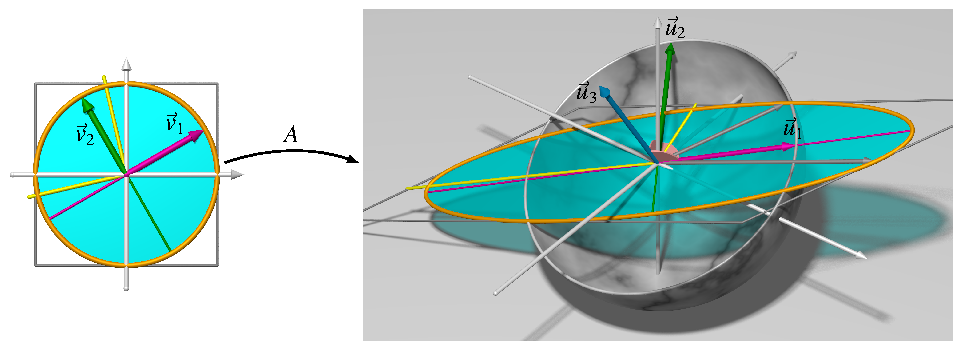
\includegraphics[width=\textwidth]{7/images/svdmotivation.pdf}
\caption{
Konstruktion der Singulärwertzerlegung einer linearen Abbildung mit
der Matrix $A$.
$A$ bildet den Einheitskreis in $\mathbb{R}^2$ auf eine Ellipse
in $\mathbb{R}^3$ ab.
Die Länge der Halbachsen der Ellipse sind die Singulärwerte $s_1$ und $s_2$ 
von $A$.
Die Richtungen $\vec{u}_1$ und $\vec{u}_2$  der Halbachsen 
können durch $\vec{u}_3$ zu einer orthonormierten Basis von
$\mathbb{R}^3$ ergänzt werden.
Die Vektoren $\vec{v}_1$ und $\vec{v}_2$ werden von $A$ auf die
Halbachsenrichtungen $\vec{u}_1$ und $\vec{u}_2$ abgebildet.
Die Singulärwertzerlegung erhält man dann, indem man die Vektoren 
$\vec{v}_i$ als Spalten in eine Matrix $V$ und die Vektoren $\vec{u}_j$
als Spalten in eine Matrix $U$ schreibt.
Zusammen mit der Matrix $S$ aus \eqref{eqn:svd:Smatrix} erhält man
die Zerlegung $A=USV^t$.
\label{figure:svdmotivation}
}
\end{figure}

Das Produkt $V^t\vec{x}$ liefert die Koordinaten von $\vec{x}$
bezüglich der Basis $\mathcal{V}$.
Diese Koordinaten werden jetzt um die Faktoren $s_1$ und $s_2$ 
gestreckt und sollen die Koordinaten eines Punktes in $\mathbb{R}^3$
bezüglich der Basis $\mathcal{U}=\{\vec{u}_1,\vec{u}_2,\vec{u}_3\}$ ergeben.
Die $\vec{u}_3$-Komponente ist immer $0$, daher ist die zu diesem
Schritt gehörige Abbildungsmatrix
\begin{equation}
S=\begin{pmatrix}
s_1& 0 \\
 0 &s_2\\
 0 & 0
\end{pmatrix}.
\label{eqn:svd:Smatrix}
\end{equation}

Die Koordinaten $SV^t\vec{x}$ bezüglich der Basis $\mathcal{U}$
müssen jetzt in einen Vektor in $\mathbb{R}^3$ umgerechnet werden.
Schreibt man die Vektoren $\vec{u}_i$ in die Spalten der Matrix $U$,
dann wird dies durch das Produkt $USV^t\vec{x}$ erreicht.
Da $\mathcal{U}$ eine Orthonormalbasis ist, ist $U$ eine orthogonale
Matrix.


\begin{satz}[Singulärwertzerlegung]\label{satz-svd}
Sei $A$ eine $m\times n$-Matrix mit Rang $r$.
Dann gibt es eine orthogonale $m\times m$-Matrix $U$, eine
orthogonale $n\times n$-Matrix $V$ und eine $m\times n$-Diagonalmatrix
mit Rang $r$ 
\begin{equation}
S=\left(
\begin{tabular}{>{$}c<{$}>{$}c<{$}>{$}c<{$}|>{$}c<{$}>{$}c<{$}>{$}c<{$}}
s_1   &\dots &0     &0     &\dots &0\\
\vdots&\ddots&\vdots&\vdots&\ddots&\vdots\\
0     &\dots &s_r   &0     &\dots &0\\
\hline
0     &\dots &0     &0     &\dots &0\\
\vdots&\ddots&\vdots&\vdots&\ddots&\vdots\\
0     &\dots &0     &0     &\dots &0\\
\end{tabular}
\right)
\label{s-matrix}
\end{equation}
mit $s_1\ge s_2\ge\dots \ge s_r$ und $A=USV^t$.
\end{satz}

\subsection{Berechnung der Singulärwertzerlegung
\label{subsection:berechnungdersingulaerwertzerleung}}
Im folgenden nehmen wir an, dass die Matrix $A$ eine Singulärwertzerlegung
$A=USV^t$ hat.
Das Produkt $A^tA$ ist
\[
A^tA
=
(USV^t)^tUSV^t
=
VS^t\underbrace{U^tU}_{=E}SV^t
=
VS^tSV^t
=
V
\begin{pmatrix}
s_1^2 &  0   & \dots &  0   &  0   &\dots\\
  0   &s_2^2 & \dots &  0   &  0   &\dots\\
\vdots&\vdots&\ddots &\vdots&\vdots&     \\
  0   &  0   & \dots & s_r^2&  0   &\dots\\
  0   &  0   & \dots &   0  &  0   &\dots\\
\vdots&\vdots&       &\vdots&\vdots&\ddots
\end{pmatrix}
V^t
\]
Die orthogonale Matrix $V^t$ transformiert also die symmetrische Matrix
$A^tA$ auf Diagonalform.
In der Eigenwertheorie (Kapitel~\ref{chapter-eigen}) wird gezeigt,
dass es zu jeder symmetrischen Matrix eine orthogonale Matrix
gibt, die sie auf Diagonalform transformiert
(Satz~\ref{satz:symmetrischdiagonalisierbar}).
In den Spalten der Matrix $V$ stehen dann Eigenvektoren von $A^tA$,
die Eigenwerte sind die $s_i^2$ oder $0$.

Für die Matrix $U$ gilt natürlich dasselbe.
Das Produkt
\[
AA^t
=
USV^tVS^tU^t
=
USS^tU^t
\]
zeigt, dass $U^t$ die symmetrische Matrix $AA^t$ auf Diagonalform
transformiert.

Die Matrizen $U$ und $V$ sind allerdings nicht eindeutig.
Dies kann man schon am Motivationsbeispiel in
Abbildung~\ref{figure:svdmotivation} erkennen.
Die Vektoren $\vec{u}_1$ und $\vec{u}_2$ waren als die Richtungen
der grössten und kleinsten Ausdehnung der Ellipse festgelegt,
aber $-\vec{u}_1$ und $-\vec{u}_2$ erfüllen diese Bedingung auch.
Wenn zwei Singulärwerte gleich sind, zum Beispiel weil sie 0 sind,
dann kann man eine beliebige Drehung in der von den Vektoren aufgespannten
Ebene durchführen und erhält ebenfalls anwendbare Vektoren.
Man muss daher separat sicherstellen, dass die $\vec{u}_i$ tatsächlich
die Bilder der Vektoren $\vec{v}_i$ unter der Abbildung $A$ sind.
Am einfachsten geht dies, wenn man den folgenden Algorithmus verwendet:
\begin{enumerate}
\item
Bestimme Vektoren $\vec{v}_i$ als Eigenvektoren von $A^tA$ mit
Eigenwerten $\lambda_i$.
Die Vektoren sollen so geordnet sein, dass 
\[
\lambda_1 \ge \lambda_2 \ge \dots \ge \lambda_r > 0
\]
gilt.
\item
Die Singulärwerte sind $s_i = \sqrt{\lambda_i}$
\item
Wähle $\vec{u}_i=A\vec{v}_i/|A\vec{v}_i|$ für $1\le i\le r$
\item
Wähle eine beliebige orthonormierte Basis von $\operatorname{ker} AA^t$
für die Vektoren $\vec{u}_{r+1},\dots,\vec{u}_m$.
\end{enumerate}
Für die Bestimmung der Eigenwerte und Vektoren wird auf
Kapitel~\ref{chapter-eigen} verweisen.

Die Berechnung der Singulärwertzerlegung kann in Octave/Matlab
mit der Funktion {\tt svd} erfolgen.
Sie liefert einen Vektor mit den Singulärwerten $s_1,\dots,s_n$ zurück.
Will man auch die Matrizen $U$ und $V$ bekommen, muss man als Rückgabewert
eine Matrix von Rückgabewerten spezifizieren
\begin{verbatim}
[U, S, V] = svd(A)
\end{verbatim}

\begin{beispiel}
Die Singulärwertzerlegung der Matrix $A$ aus dem letzten Beispiel 
bekommt man mit Octave:
\begin{verbatim}
> [U,S,V] = svd([9,3,3;3,17,21;3,21,107])
U =

   0.034813  -0.443841   0.895429
   0.217231  -0.871189  -0.440272
   0.975499   0.209842   0.066088

S =

Diagonal Matrix

   111.7835          0          0
          0    13.4702          0
          0          0     7.7464

V =

   0.034813  -0.443841   0.895429
   0.217231  -0.871189  -0.440272
   0.975499   0.209842   0.066088
\end{verbatim}
\end{beispiel}
\subsection{Pseudoinverse}
\index{Pseudoinverse}
Als Anwendung der Singulärwertzerlegung betrachten wir das Problem, eine Matrix
$A^\dagger$
zu finden, die ``so inverse wie möglich'' ist zu einer gegebenen
$n\times m$-Matrix $A$.
Natürlich können wir nicht erwarten, dass das Produkt $AA^\dagger$ 
oder $A^\dagger A$
eine Einheitsmatrix ergibt.
Wenn die Matrix $A$ den Rang $r$ hat, dann sollte auch $A^\dagger$ den Rang $r$
haben.
Ist der Rang nicht voll, dann könnten wir erwarten, dass das Produkt die Form
\[
P=
\begin{pmatrix}
1&      & & &      & \\
 &\ddots& & &      & \\
 &      &1& &      & \\
 &      & &0&      & \\
 &      & & &\ddots& \\
 &      & & &      &0\\
\end{pmatrix}
\]
mit genau $r$ Einsen in der linken oberen Ecke hat.
Man nennt $P$ eine {\em Projektionsmatrix}, sie hat die Eigenschaft $P^2=P$.
\index{Projektion}
\index{Projektionsmatrix}
Dies ist aber zu viel verlangt, ändert man nämlich das Koordinatensystem,
dann geht die spezielle Form der Matrix $P$ verloren.
Die Projektionseigenschaft $P^2=P$ ist jedoch unabhängig vom Koordinatensystem.
Ist nämlich $T$ eine Transformationsmatrix und $P'=TPT^{-1}$, dann gilt
\[
P'^2=TPT^{-1}TPT^{-1}=TPPT^{-1}=TPT^{-1}=P'.
\]

\begin{beispiel}
Die Matrix
\[
P=\begin{pmatrix}1&0\\0&0\end{pmatrix}
\]
ist eine Projektionsmatrix.
Dreht man das Koordinatensystem um den Winkel $\alpha$, wird die Matrix 
gemäss $P'=D_\alpha AD_\alpha ^{-1}=D_\alpha AD_\alpha^t$ transformiert:
\begin{align*}
P'&=
\begin{pmatrix}\cos\alpha&-\sin\alpha\\\sin\alpha&\cos\alpha\end{pmatrix}
\begin{pmatrix}1&0\\0&0\end{pmatrix}
\begin{pmatrix}\cos\alpha&\sin\alpha\\-\sin\alpha&\cos\alpha\end{pmatrix}
\\
&=
\begin{pmatrix}\cos\alpha&-\sin\alpha\\\sin\alpha&\cos\alpha\end{pmatrix}
\begin{pmatrix}\cos\alpha&\sin\alpha\\0&0\end{pmatrix}
\\
&=
\begin{pmatrix}\cos^2\alpha&\cos\alpha\sin\alpha\\\sin\alpha\cos\alpha&\sin^2\alpha\end{pmatrix}.
\end{align*}
Wir kontrollieren die Projektionseigenschaft:
\begin{align*}
P^{\prime 2}
&=
\begin{pmatrix}
\cos^2\alpha
	&\sin\alpha\cos\alpha\\
\sin\alpha\cos\alpha
	&\sin^2\alpha
\end{pmatrix}^2
\\
&=
\begin{pmatrix}
\cos^4\alpha + \sin^2\alpha\cos^2\alpha
	&\sin\alpha\cos^3\alpha+\sin^3\alpha\cos\alpha\\
\sin\alpha\cos^3\alpha+\sin^3\alpha\cos\alpha
	&\sin^2\alpha\cos^2\alpha+\sin^4\alpha
\end{pmatrix}
\\
&=
\begin{pmatrix}
(\cos^2\alpha + \sin^2\alpha)\cos^2\alpha
	&\sin\alpha\cos\alpha(\cos^2\alpha+\sin^2\alpha)\\
\sin\alpha\cos\alpha(\cos^2\alpha+\sin^2\alpha)
	&\sin^2\alpha(\cos^2\alpha+\sin^2\alpha)
\end{pmatrix}
\\
&=
\begin{pmatrix}
\cos^2\alpha
	&\sin\alpha\cos\alpha\\
\sin\alpha\cos\alpha
	&\sin^2\alpha
\end{pmatrix}=P'.
\end{align*}
\end{beispiel}

Wir können also nur erwarten, dass $A^\dagger A$ bzw.~$AA^\dagger$ die
Projektionseigenschaft haben.
Nur im Falle vollen Ranges wird eines der Produkte eine Einheitsmatrix sein.

In einfachen Fällen können wir eine Pseudoinverse sofort angeben.
Die Matrix $A$
\[
A=\begin{pmatrix}
2&0&0\\
0&3&0\\
0&0&0
\end{pmatrix}
\]
ist nicht invertierbar, weil sie nicht vollen Rang hat.
Aber die Matrix
\[
A^\dagger=\begin{pmatrix}
\frac12&0&0\\
0&\frac13&0\\
0&0&0
\end{pmatrix}
\]
ist in dem Sinne eine Inverse, dass $AA^{\dagger}$ und $A^\dagger A$ zwar keine
Einheitsmatrizen sind, aber doch mindestens Projektionsmatrizen mit dem gleichen
Rang wie $A$:
\begin{align*}
AA^\dagger=A^\dagger A
=
\begin{pmatrix}
1&0&0\\
0&1&0\\
0&0&0
\end{pmatrix}.
\end{align*}
Diesen Spezialfall wollen wir im Folgenden verallgemeinern.

Eine $m\times n$-Diagonalmatrix $S$ wie in (\ref{s-matrix}) in Satz~\ref{satz-svd}
hat als Pseudoinverse die $n\times m$-Matrix
\begin{equation}
S^\dagger=\left(
\begin{tabular}{>{$\displaystyle}c<{$}>{$\displaystyle}c<{$}>{$\displaystyle}c<{$}>{$\displaystyle}c<{$}|>{$}c<{$}>{$}c<{$}>{$}c<{$}}
\frac1{s_1}&           &      &           &     &      & \\
           &\frac1{s_2}&      &           &     &      & \\
           &           &\ddots&           &     &      & \\
           &           &      &\frac1{s_r}&     &      & \\
\hline
           &           &      &           &\quad&      & \\
           &           &      &           &     &     0& \\
           &           &      &           &     &      &\qquad
\end{tabular}
\right)
\end{equation}
denn die Produkte $S^\dagger S$ und $SS^\dagger$ sind beide Projektionsmatrizen
mit Rang $r$.
$S^\dagger S$ ist eine $n\times n$-Matrix, $SS^\dagger$ ist eine
$m\times m$-Matrix.

Mit Hilfe der Singulärwertzerlegung lässt sich diese Konstruktion
auf beliebige Matrizen verallgemeinern.
Sei $A$ eine $m\times n$-Matrix mit Singulärwertzerlegung
$A=USV^t$, wobei $U$ eine orthogonale $m\times m$-Matrix, $V$ eine orthogonale
$n\times n$-Matrix und $S$ eine $m\times n$-Diagonalmatrix wie in (\ref{s-matrix})
von Satz~\ref{satz-svd} ist.
Wir setzen
\begin{equation}
A^\dagger = VS^\dagger U^t,
\label{definition-pseudoinverse}
\end{equation}
$A^\dagger$ heisst die {\em Pseudoinverse} von $A$.

Wir überzeugen uns zunächst, dass $A^\dagger$ für invertierbare Matrizen
mit der gewöhnlichen Inversen $A^{-1}$ übereinstimmt.
Für invertierbares $A$ ist $n=m$ und $S$ ist eine Diagonalmatrix ohne Nullen
auf der Diagonalen.
Insbesondere gilt $S^\dagger=S^{-1}$, oder $S^\dagger S=SS^\dagger=E$.
Daher gilt auch
\begin{align*}
A^\dagger A&=VS^\dagger U^tUSV^t=VS^\dagger SV^t=VV^t=E\\
AA^\dagger &=USV^tVS^\dagger U^t=USS^\dagger U^t=UU^t=E,
\end{align*}
also ist $A^\dagger=A^{-1}$ in diesem Fall.

Im allgemeinen Fall gilt
\begin{align*}
A^\dagger A&=VS^\dagger U^tUSV^t=VS^\dagger SV^t=VP_1V^{-1}\\
AA^\dagger &=USV^tVS^\dagger U^t=USS^\dagger U^t=UP_2U^{-1},
\end{align*}
wobei die $P_i$ geeignete Projektionsmatrizen sind.
In einem geeigneten Koordinatensystem, das im Wesentlichen durch die Matrizen
$U$ bzw.~$V$ gegeben ist, sind die Produkte $A^\dagger A$ und $AA^\dagger$
also Projektionsmatrizen.
Anders ausgedrückt, soweit es möglich ist, also in den durch die Projektion
gegebenen Unterräumen, ist $A^\dagger$ eine Inverse von $A$.
$A^\dagger$ heisst die {\em Pseudoinverse} von $A$.

\begin{beispiel}
Die Matrix
\[
A=\begin{pmatrix}
1&2&9&1\\
2&0&1&5
\end{pmatrix}
\]
hat Rang $2$.
Wir berechnen die Pseudoinverse mit Hilfe von Octave, dazu bestimmen wir
zunächst die Singulärwertzerlegung:
\begin{verbatim}
> A = [1,2,9,1;2,0,1,5]
A =

   1   2   9   1
   2   0   1   5

> [U,S,V] = svd(A)
U =

  -0.96747  -0.25300
  -0.25300   0.96747

S =

Diagonal Matrix

   9.5490        0        0        0
        0   5.0809        0        0

V =

  -0.154305   0.331029  -0.751912  -0.548852
  -0.202631  -0.099587  -0.575830   0.785775
  -0.938335  -0.257732   0.182137  -0.141163
  -0.233789   0.902262   0.264337   0.247774
\end{verbatim}
Aus $S$ können wir jetzt die Pseudoinverse $S^\dagger$ berechnen:
\begin{verbatim}
> Sdagger = S';
> Sdagger(1,1)=1/S(1,1);
> Sdagger(2,2)=1/S(2,2)
Sdagger =

Diagonal Matrix

   0.10472         0
         0   0.19681
         0         0
         0         0
\end{verbatim}
Wir kontrollieren, ob sie die verlangte Projektionseigenschaft hat:
\begin{verbatim}
> Sdagger * S
ans =

Diagonal Matrix

   1   0   0   0
   0   1   0   0
   0   0   0   0
   0   0   0   0

> S * Sdagger
ans =

Diagonal Matrix

   1   0
   0   1
\end{verbatim}
Jetzt können wir mit Hilfe der Matrizen $U$ und $V$ auch die Pseudoinverse
$A^\dagger$ bestimmen.
\begin{verbatim}

> Adagger = V * Sdagger * U'
Adagger =

  -8.4962e-04   6.7120e-02
   2.5489e-02  -1.3594e-02
   1.0790e-01  -2.4214e-02
  -2.1240e-02   1.7799e-01

\end{verbatim}
Das Produkt $AA^\dagger$ muss eine Projektionsmatrix vom Rang $2$ sein, wir
berechnen
\begin{verbatim}
> A * Adagger
ans =

   1.0000e+00  -5.5511e-17
  -2.7756e-17   1.0000e+00
\end{verbatim}
im Rahmen der Rechengenauigkeit ist das tatsächlich eine Einheitsmatrix.

Das Produkt $A^\dagger A$ muss eine Projektionsmatrix sein, es muss also
für $P=A^\dagger A$ gelten, dass $P^2=P$ ist.
Wir berechnen mit Octave die Differenz $P^2-P$ und erhalten
\begin{verbatim}
> P = Adagger * A
P =

   0.1333900  -0.0016992   0.0594732   0.3347494
  -0.0016992   0.0509771   0.2158029  -0.0424809
   0.0594732   0.2158029   0.9468989  -0.0131691
   0.3347494  -0.0424809  -0.0131691   0.8687341

> P * P - P
ans =

   5.5511e-17  -1.7347e-18   1.3878e-17   1.1102e-16
  -1.2143e-17   6.9389e-18   0.0000e+00  -2.7756e-17
  -2.0817e-17   0.0000e+00   1.1102e-16  -7.2858e-17
   1.1102e-16  -1.3878e-17   0.0000e+00   3.3307e-16
\end{verbatim}
Im Rahmen der Rechengenauigkeit ist das $0$.
\end{beispiel}


